% Draft: Methodology (as built), Experimental Setup, Results skeleton, Limitations.
% Written 2026-10-02 from experiments/README.md, experiments/DECISIONS.md and the code.
% Not \input by main.tex: the author merges what they keep. Every number comes
% from \result{...} (paper/generated/results.tex, preamble: % generated by experiments/export_paper.sh — do not edit
% generated by experiments/e0_instruments/run.py, 2026-10-05T21:34:43-03:00, git 92dd644 — do not edit
\makeatletter
\providecommand\result[1]{\@ifundefined{result@#1}{\PackageError{results}{Unknown result key `#1'}{Run the experiment, then experiments/export_paper.sh.}}{\@nameuse{result@#1}}}
\@namedef{result@e0/demo1/arcface.genuine-mean}{0.455}
\@namedef{result@e0/demo1/arcface.impostor-mean}{0.104}
\@namedef{result@e0/demo1/arcface.tar}{0.319}
\@namedef{result@e0/demo1/arcface.threshold}{0.616}
\@namedef{result@e0/demo1/facenet.genuine-mean}{0.559}
\@namedef{result@e0/demo1/facenet.impostor-mean}{0.268}
\@namedef{result@e0/demo1/facenet.tar}{0.187}
\@namedef{result@e0/demo1/facenet.threshold}{0.814}
\@namedef{result@e0/demo2/arcface.genuine-mean}{0.614}
\@namedef{result@e0/demo2/arcface.impostor-mean}{0.173}
\@namedef{result@e0/demo2/arcface.tar}{0.650}
\@namedef{result@e0/demo2/arcface.threshold}{0.542}
\@namedef{result@e0/demo2/facenet.genuine-mean}{0.784}
\@namedef{result@e0/demo2/facenet.impostor-mean}{0.350}
\@namedef{result@e0/demo2/facenet.tar}{0.638}
\@namedef{result@e0/demo2/facenet.threshold}{0.784}
\@namedef{result@e0/demo3/arcface.genuine-mean}{0.570}
\@namedef{result@e0/demo3/arcface.impostor-mean}{0.165}
\@namedef{result@e0/demo3/arcface.tar}{0.586}
\@namedef{result@e0/demo3/arcface.threshold}{0.522}
\@namedef{result@e0/demo3/facenet.genuine-mean}{0.742}
\@namedef{result@e0/demo3/facenet.impostor-mean}{0.290}
\@namedef{result@e0/demo3/facenet.tar}{0.634}
\@namedef{result@e0/demo3/facenet.threshold}{0.713}
\@namedef{result@e0/mechanism/emap-direction-cos-mean}{-0.027}
\@namedef{result@e0/mechanism/emap-orthogonality}{51.870}
\@namedef{result@e0/mechanism/faces}{300}
\@namedef{result@e0/mechanism/recognizer-cos-mean}{1.000}
\@namedef{result@e0/mechanism/recognizer-cos-min}{1.000}
\@namedef{result@e0/noise/age_err}{1.178}
\@namedef{result@e0/noise/age_err.ci}{0.192}
\@namedef{result@e0/noise/arcface.cos}{0.923}
\@namedef{result@e0/noise/arcface.cos.ci}{0.015}
\@namedef{result@e0/noise/emotion_agree}{0.948}
\@namedef{result@e0/noise/emotion_agree.ci}{0.021}
\@namedef{result@e0/noise/emotion_kappa}{0.860}
\@namedef{result@e0/noise/emotion_kappa.ci}{0.054}
\@namedef{result@e0/noise/expression}{0.032}
\@namedef{result@e0/noise/expression.ci}{0.008}
\@namedef{result@e0/noise/facenet.cos}{0.959}
\@namedef{result@e0/noise/facenet.cos.ci}{0.008}
\@namedef{result@e0/noise/gender_agree}{0.940}
\@namedef{result@e0/noise/gender_agree.ci}{0.019}
\@namedef{result@e0/noise/pose_err}{1.968}
\@namedef{result@e0/noise/pose_err.ci}{0.361}
\makeatother

),
% so this compiles only after experiments/export_paper.sh; a missing key stops
% the compilation on purpose. "% TODO" marks a sentence to write once the
% numbers are known; nothing here anticipates a result.

\section{Methodology}

The framework is an offline, three-stage pipeline: (1)~face detection and
tracking with a recall post-pass, (2)~per-track face replacement by a
generative model, and (3)~a fail-closed composition of the output video.
Temporal consistency is obtained by fixing one synthetic identity per track
rather than by a separate stabilization network.

\subsection{Stage 1: detection, tracking and recall}

Faces are detected by SCRFD-10GF~\cite{scrfd} (InsightFace's \texttt{buffalo\_l}
pack, inference only, 640\,px input) and associated across frames by a
ByteTrack-style tracker: detections at or above 0.5 are matched first and may
start new tracks, while detections between 0.1 and 0.5 can only extend an
existing track, which recovers partially occluded or bowed faces without
creating spurious tracks. Because the pipeline is offline, a post-pass over the
whole video then places a box wherever a tracked face almost certainly is:
tracks are emitted from their first detection rather than after a
confirmation delay, gaps of up to 30 frames inside a track are filled by
linear interpolation, each track is extended by three frames at both ends, and
tracks with fewer than three detections are kept for hiding but receive no
synthetic identity. Every box records its origin (detector, interpolated,
dilated, unconfirmed); only detector boxes, which carry landmarks, reach the
generator.

% Note for the text: the SCRFD-10GF threshold defaulted to 0.5 inside InsightFace
% regardless of the configured value before 2026-09-30 (DECISIONS.md 35); every
% number in this draft uses the corrected pipeline.

\subsection{Stage 2: face replacement}

Three generator families are compared in their published form: CIAGAN~\cite{ciagan}
(a conditional GAN driven by landmarks and a one-hot identity code),
GANonymization~\cite{hellmann} (pix2pix re-synthesis from dense landmarks) and
BLANKET (an SDXL inpainting model with two ControlNets that generates one
synthetic identity per track, followed by an \texttt{inswapper} face swap in
every frame). Blur and mosaic of the detected box are the censorship baselines.
Each track receives a deterministic seed, so a student keeps one pseudonymous
face throughout the video.

Our contribution modifies the replacement in four places. \textbf{(C2) Track-level
real identity.} For every track, the ArcFace (\texttt{w600k\_r50}) embeddings of
its frames are aggregated into one estimate of the real person's identity,
weighted by a quality score (detection confidence, face size, head yaw) with
outlier gating; it also selects the best frames from which the synthetic
identity is generated. \textbf{(P2) Swap-stage push.} The identity embedding
that conditions the swap is moved away from that estimate,
$\hat{e} = \mathrm{normalize}(e_{\mathrm{synth}} - \beta\, e_{\mathrm{real}})$,
in the same space before \texttt{inswapper}'s projection, replacing BLANKET's
fixed single-frame mix. \textbf{(P3) CIAGAN code optimization.} Per frame, a few
gradient steps move CIAGAN's identity code (a softmax over its 1200 training
identities, initialized at the track's seed) to reduce
$\max(0, \cos(\mathrm{ArcFace}(x), e_{\mathrm{real}}) - \tau)$, with a penalty
that keeps the code near the seed's pseudonym. \textbf{(P1) Diffusion guidance.}
During BLANKET's identity generation, the predicted clean latent is pushed by
the gradient of the same hinge through a differentiable ArcFace, in the manner
of MPGD, without back-propagating through the denoising network.
% TODO P1: keep or move to future work after the go/no-go spike (DECISIONS.md 44).

Two engineering changes made BLANKET usable on classroom footage. The swap uses
the face Stage~1 found (its box and five landmarks) instead of re-detecting it,
and identity images the swapper's detector rejects are re-examined with a
more permissive detector; on one video these two changes raised the share of
generated faces from 0.43 to 1.0 on the same identities (frames 0--99).
% TODO: replace with the E3b numbers (\result{e3b/pooled/phase1/anonymized}).

\subsection{Stage 3: fail-closed composition}

The output video never shows a face the pipeline knows about. Generated faces
are pasted back pixel-exactly (only the pixels the generator changed, so a
neighbour's background cannot overwrite them); every other box---a generation
failure, a post-pass box, a rejected swap---is hidden by the same track's most
recent generated face (if at most 10 frames old) or by a neutral gray ellipse.
Blur and pixelation are not used as the fallback, since both are reversible or
attackable for small faces.

\section{Experimental Setup}

\textbf{Data.} Detection is benchmarked on the WIDER FACE validation split with
the official protocol. The video experiments use three classroom recordings
(239, 244 and 355 frames) with 15, 24 and 22--32 tracks, respectively.
% TODO: state the source and terms of the three videos, and that no frame of a
% real person is reproduced in this paper; they are not a consented dataset of
% children (limitation).

\textbf{Privacy.} Two recognizers are reported side by side: FaceNet
(InceptionResnetV1 trained on VGGFace2), a held-out evaluator never used to
build or steer the pipeline, and ArcFace (\texttt{w600k\_r50}), the space in
which P1--P3 push. Thresholds are calibrated in-domain, per video, at a 1\%
false-accept rate, with genuine pairs from the same track and impostor pairs
from tracks visible in the same frame. Re-identification is closed-set: each
face is compared with the mean real embedding of every track (its own frame
left out), and rank-1/rank-5 record whether its own track ranks first or in the
top five; Privacy Gain is $1 - \mathrm{rank1}_{\mathrm{anon}} / \mathrm{rank1}_{\mathrm{real}}$.
Each metric is computed in three views: generated faces only (the generator's
quality), all faces with passthrough counted as a leak (the method as
published), and the final video after the fail-safe (what a viewer sees). The
primary measure is FaceNet rank-1 on the final video.

\textbf{Utility.} Between each real face and its replacement: emotion agreement
(8 classes, HSEmotion), expression error (106 landmarks after similarity
alignment, in inter-ocular units), head-pose error (mean absolute error of
pitch, yaw and roll), age error and gender agreement (InsightFace), and
re-detection. Each is read against its noise floor, the same metric between
consecutive real frames of a track (Table~\ref{tab:noise}).

\textbf{Statistics.} Confidence intervals (95\%) are percentile bootstraps that
resample whole tracks; arms that share faces are compared on the same faces,
with a track-level sign-flip test. Results are pooled over the three videos and
stratified by face size, absolute yaw and detection confidence.

\textbf{Criteria, fixed before running.} An arm improves privacy when FaceNet
rank-1 drops and the paired interval against its reference excludes zero; it
preserves utility when its utility metrics stay within the reference arm's
interval, read against the noise floor.

\section{Results}

\subsection{Instruments}

\begin{table}[ht]\centering
\caption{Recognizers on real faces of each video: in-domain threshold and true-accept rate at FAR 1\%.}
\label{tab:recognizers}
% generated by experiments/e0_instruments/run.py — do not edit
\begin{tabular}{llrrrrr}
\toprule
Video & Recognizer & Threshold & TAR & Genuine & Impostor & Pairs \\
\midrule
demo1 & FaceNet & 0.776 & 0.353 & 0.649 & 0.282 & 436/2300 \\
demo1 & ArcFace & 0.471 & 0.587 & 0.531 & 0.057 & 436/2300 \\
demo2 & FaceNet & 0.777 & 0.692 & 0.808 & 0.331 & 996/10500 \\
demo2 & ArcFace & 0.527 & 0.795 & 0.672 & 0.158 & 996/10500 \\
demo3 & FaceNet & 0.713 & 0.731 & 0.785 & 0.285 & 1327/17450 \\
demo3 & ArcFace & 0.531 & 0.741 & 0.661 & 0.163 & 1327/17450 \\
\bottomrule
\end{tabular}

\end{table}

\begin{table}[ht]\centering
\caption{Noise floor of the utility metrics: the same metric between consecutive real frames.}
\label{tab:noise}
% generated by experiments/e0_instruments/run.py — do not edit
\begin{tabular}{lrr}
\toprule
Metric (consecutive real frames) & Value & Pairs \\
\midrule
Expression error & 0.032\,{\scriptsize$\pm$0.008} & 12529 \\
Head-pose error (\textdegree{}) & 1.968\,{\scriptsize$\pm$0.361} & 12529 \\
Emotion agreement & 0.948\,{\scriptsize$\pm$0.021} & 12529 \\
Emotion agreement (Cohen's $\kappa$) & 0.860\,{\scriptsize$\pm$0.054} & 12529 \\
Age difference (years) & 1.178\,{\scriptsize$\pm$0.192} & 12529 \\
Gender agreement & 0.940\,{\scriptsize$\pm$0.019} & 12529 \\
FaceNet cosine & 0.959\,{\scriptsize$\pm$0.008} & 12529 \\
ArcFace cosine & 0.923\,{\scriptsize$\pm$0.015} & 12529 \\
\bottomrule
\end{tabular}

\end{table}

FaceNet accepts \result{e0/demo2/facenet.tar} of genuine pairs on demo2 and
\result{e0/demo1/facenet.tar} on demo1 at FAR 1\%.
% TODO: interpret the evaluator's validity per video (demo1 is the weakest).

\subsection{Detection}

\begin{table}[ht]\centering
\caption{WIDER FACE validation: official AP and inference cost.}
\label{tab:wider}
% generated by experiments/e1_detection/run.py — do not edit
\begin{tabular}{lrrrrr}
\toprule
Detector & AP easy & AP medium & AP hard & Latency (ms) & Params (M) \\
\midrule
SCRFD-10GF & 0.949 & 0.935 & 0.813 & \textbf{21.540} & 4.230 \\
SCRFD-34GF & 0.959 & 0.947 & 0.840 & 40.670 & 9.780 \\
YOLO-FaceV2-s & \textbf{0.987} & \textbf{0.973} & \textbf{0.894} & 177.330 & 7.050 \\
\bottomrule
\end{tabular}

\end{table}

\begin{table}[ht]\centering
\caption{Recall-first operating points on WIDER FACE (hard set).}
\label{tab:wider-recall}
% generated by experiments/e1_detection/run.py — do not edit
\begin{tabular}{lrrrrr}
\toprule
Detector & P @ 0.3 & R @ 0.3 & F1 @ 0.3 & R @ FPPI 0.01 & R @ FPPI 0.1 \\
\midrule
SCRFD-10GF & 0.835 & 0.769 & 0.800 & 0.375 & 0.562 \\
SCRFD-34GF & 0.835 & 0.797 & 0.816 & 0.391 & 0.584 \\
YOLO-FaceV2-s & 0.858 & \textbf{0.865} & 0.861 & \textbf{0.419} & \textbf{0.678} \\
\bottomrule
\end{tabular}

\end{table}

SCRFD-10GF reaches an AP of \result{e1/widerface/scrfd-10gf/ap-hard} on the hard
set and a recall of \result{e1/widerface/scrfd-10gf/recall-at-fppi-0.1} at 0.1
false positives per image.
% TODO: compare detectors; Table e1-videos (track statistics) for the classroom videos.

\subsection{Generators in their original form}

\begin{table}[ht]\centering
\caption{Privacy, pooled over videos: coverage and FaceNet rank-1 in three views
(generated faces, all faces with passthrough as a leak, final video), Privacy Gain
and verification on the final video. Mean $\pm$ half-width of the 95\% track bootstrap.}
\label{tab:e2-main}
% generated by experiments/e2_generation/run.py — do not edit
\begin{tabular}{@{}l@{\hspace{5pt}}r@{\hspace{5pt}}r@{\hspace{5pt}}r@{\hspace{5pt}}r@{\hspace{5pt}}r@{\hspace{5pt}}r@{}}
\toprule
Arm & Coverage & R1 gen. & R1 all & R1 final & PG final & Verified \\
\midrule
blur & 1.00\,{\scriptsize$\pm$.00} & 0.07\,{\scriptsize$\pm$.05} & 0.07\,{\scriptsize$\pm$.05} & \textbf{0.07\,{\scriptsize$\pm$.05}} & 0.92\,{\scriptsize$\pm$.06} & 0.01\,{\scriptsize$\pm$.01} \\
mosaic & 1.00\,{\scriptsize$\pm$.00} & 0.12\,{\scriptsize$\pm$.06} & 0.12\,{\scriptsize$\pm$.06} & 0.12\,{\scriptsize$\pm$.06} & 0.87\,{\scriptsize$\pm$.07} & 0.02\,{\scriptsize$\pm$.01} \\
ciagan & 1.00\,{\scriptsize$\pm$.00} & 0.08\,{\scriptsize$\pm$.04} & 0.08\,{\scriptsize$\pm$.04} & 0.08\,{\scriptsize$\pm$.04} & 0.91\,{\scriptsize$\pm$.05} & \textbf{0.00\,{\scriptsize$\pm$.00}} \\
ganonymization & 0.47\,{\scriptsize$\pm$.10} & 0.10\,{\scriptsize$\pm$.06} & 0.51\,{\scriptsize$\pm$.10} & 0.09\,{\scriptsize$\pm$.04} & 0.90\,{\scriptsize$\pm$.04} & 0.03\,{\scriptsize$\pm$.02} \\
blanket & 0.28\,{\scriptsize$\pm$.12} & 0.48\,{\scriptsize$\pm$.16} & 0.77\,{\scriptsize$\pm$.07} & 0.15\,{\scriptsize$\pm$.08} & 0.84\,{\scriptsize$\pm$.09} & 0.02\,{\scriptsize$\pm$.02} \\
\bottomrule
\end{tabular}

\end{table}

\begin{table}[ht]\centering
\caption{Utility on generated faces, with the noise floor (real, next frame).}
\label{tab:e2-utility}
% generated by experiments/e2_generation/run.py — do not edit
\begin{tabular}{@{}l@{\hspace{5pt}}r@{\hspace{5pt}}r@{\hspace{5pt}}r@{\hspace{5pt}}r@{\hspace{5pt}}r@{\hspace{5pt}}r@{}}
\toprule
Arm & Expr. & Pose (\textdegree{}) & Emotion $\kappa$ & Age (y) & Gender & Re-det. \\
\midrule
blur & 0.28\,{\scriptsize$\pm$.04} & 17.18\,{\scriptsize$\pm$1.98} & -0.01\,{\scriptsize$\pm$.02} & 7.62\,{\scriptsize$\pm$1.25} & 0.45\,{\scriptsize$\pm$.08} & 0.00\,{\scriptsize$\pm$.00} \\
mosaic & 0.23\,{\scriptsize$\pm$.05} & 16.98\,{\scriptsize$\pm$1.94} & 0.03\,{\scriptsize$\pm$.10} & 12.56\,{\scriptsize$\pm$1.99} & 0.64\,{\scriptsize$\pm$.07} & 0.00\,{\scriptsize$\pm$.00} \\
ciagan & 0.21\,{\scriptsize$\pm$.05} & 14.19\,{\scriptsize$\pm$1.75} & 0.06\,{\scriptsize$\pm$.04} & 5.92\,{\scriptsize$\pm$1.09} & 0.41\,{\scriptsize$\pm$.09} & 0.95\,{\scriptsize$\pm$.04} \\
ganonymization & 0.14\,{\scriptsize$\pm$.02} & 13.16\,{\scriptsize$\pm$1.63} & 0.08\,{\scriptsize$\pm$.07} & 31.89\,{\scriptsize$\pm$4.34} & 0.67\,{\scriptsize$\pm$.09} & 0.54\,{\scriptsize$\pm$.10} \\
blanket & 0.11\,{\scriptsize$\pm$.05} & 7.30\,{\scriptsize$\pm$2.29} & 0.12\,{\scriptsize$\pm$.10} & 5.65\,{\scriptsize$\pm$1.62} & 0.83\,{\scriptsize$\pm$.09} & 0.99\,{\scriptsize$\pm$.01} \\
Real, next frame & \textbf{0.03\,{\scriptsize$\pm$.01}} & \textbf{1.99\,{\scriptsize$\pm$.37}} & \textbf{0.86\,{\scriptsize$\pm$.05}} & \textbf{1.18\,{\scriptsize$\pm$.19}} & \textbf{0.94\,{\scriptsize$\pm$.02}} & -- \\
\bottomrule
\end{tabular}

\end{table}

\begin{figure}[ht]\centering
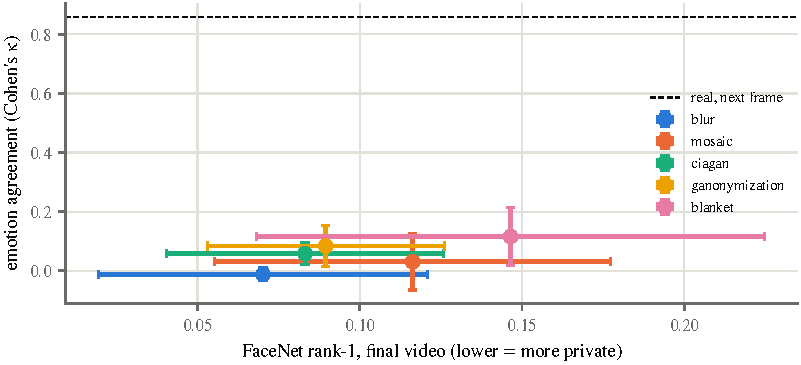
\includegraphics[width=\linewidth]{generated/e2_generation/fig-e2-tradeoff}
\caption{Privacy--utility trade-off of each method: FaceNet rank-1 on the final
video against emotion agreement; the dashed line is the noise floor.}
\label{fig:tradeoff}
\end{figure}

On the final video, FaceNet re-identifies \result{e2/pooled/blanket/facenet_final.rank1}
of BLANKET's faces, \result{e2/pooled/ciagan/facenet_final.rank1} of CIAGAN's and
\result{e2/pooled/blur/facenet_final.rank1} of the blurred ones.
% TODO: trade-off reading; strata tables (e2-strata-*); cost table (e2-cost).

\subsection{Contribution}

\begin{table}[ht]\centering
\caption{C2: estimate of the real identity per aggregation mode, scored by its
cosine to the track's unseen frames.}
\label{tab:e3-identity}
\input{generated/e3_contribution/tab-e3-identity}
\end{table}

\begin{table}[ht]\centering
\caption{P2: push strength on BLANKET (generated faces), with the paired difference
against BLANKET's own mix.}
\label{tab:e3-p2}
\input{generated/e3_contribution/tab-e3-p2-strength}
\end{table}

\begin{figure}[ht]\centering
\includegraphics[width=\linewidth]{generated/e3_contribution/fig-e3-p2-curve}
\caption{P2: rank-1 of the held-out (FaceNet) and guidance (ArcFace) recognizers,
and expression error, against the push strength $\beta$; dashed lines: BLANKET's own mix.}
\label{fig:p2}
\end{figure}

At $\beta = 1.2$, FaceNet rank-1 on generated faces changes by
\result{e3c/pooled/b-1.2/delta-facenet.rank1}~$\pm$~\result{e3c/pooled/b-1.2/delta-facenet.rank1.ci}
against BLANKET's own mix.
% TODO: transfer gap between ArcFace and FaceNet; the target table (e3-p2-target);
% P3 (e3-p3); the policies (e3-policies); P1 if kept (e3-p1).

\section{Limitations}

The three videos are not a consented dataset of children, so the study measures
the method on classroom-like footage, not on its target population. Gaze is not
measured: no permissively licensed estimator was validated on faces this small.
Human-rated pedagogical analyzability, a re-trained (parrot) attacker and a
demographic fairness analysis are not performed. The emotion classifier is
trained on AffectNet, whose terms allow research use only. Privacy is measured
against two recognizers and does not constitute a formal guarantee. Faces the
detector never finds are not hidden; their rate is estimated from annotated
frames. % TODO: \result for the residual miss rate once the frames are annotated.
